\section{View Maintenance System} 
\label{sec:view_maintenance_system} 

In this section, we present and discuss the design of \VMS. By
illustrating how a base table operation may effect a view table, we
provide the intuition for the resulting view consistency established
by \VMS.  Finally, we discuss fault-tolerance.

\subsection{Design Overview}

The lower half of Figure~\ref{fig:kv_model} gives an overview of \VMS, 
which is comprised of a \textit{master}, a number of $n$ 
\textit{source systems} (always the same number as \KVS\ nodes) and
a number of $m$ view manager. The 
input to \VMS\ is a set of operation streams; each emitted by a \KVS\ 
node (cf. Figure~\ref{fig:kv_model}). Technically, the \textit{WAL 
reader} component of a source system connects to the underlying HDFS and 
reads the WAL of its assigned node. Because operations are always 
appended to the WAL, the reading happens fast and in-order. After 
retrieving the operations from WAL, the WAL reader passes them to the 
distributor. This component distributes the incoming operation stream to 
all registered \VMs. The number of \VMs\ is configurable. \VMs\ can be 
dynamically \textit{assigned} to or \textit{removed} from the \VMS. 


A \VM\ is designed to be light-weight and can be deployed in large
numbers to accommodate a changing view update load. It computes view
updates, based on base table operations it receives as input via the
\KVS\ API, for view tables. A \VM\ only belongs to a single
sub-system. The sub-system feeds the \VM\ with operations which
processes them in order.  A \VM\ is the unit of scalability of
\VMS. \VMs\ are kept stateless to be exchangeable at any time and to
minimize dependency. Given a number of view definitions and a sequence
of operations, a \VM\ is always able to execute any view table update
from any host.

Our design exhibits at least the following four benefits: (i) Seamless
scalability: Hundreds of views may have to be updated as a consequence
of a single base table operation. As \VMS\ exceeds its service levels,
additional \VMs\ can be spawned (below, we show this
experimentally). (ii) Operational flexibility: \VMs\ introduce
flexibility to the system architecture. All \VMs\ of a given
sub-system can be hosted together on the same node or each \VM\ can be
hosted at a different node. (iii) Accommodate load variations:
\VMs\ can be reassigned from one sub-system to another as base table
update load changes. (iv) Fault-tolerance: If a \VM\ crashes, another
\VM\ can take over and continue processing the operation stream.

\subsection{Update Propagation} 
\label{subsec:update_processing} 

A source distributes the arriving base table updates (i.e. WAL stream) 
to the \VMs\ via consistent hashing by maintaining a hash-ring
(cf. Figure~\ref{fig:review_consistency}), where active \VMs\ are
registered.  Row keys of arriving updates are hashed into the ring and
associated in clock-wise direction with active \VMs.  In this way, a
source-system distributes operations uniformly across the available
\VMs\ and ensures that base table operations on the same row key are
always handled by the same \VM. On the one hand, this mechanism
ensures maximal degree of concurrency for update propagation, on the other
hand it guarantees the ordered propagation of base table
updates to view tables, setting the basis for view table consistency.

There are two alternatives to compute a the hash value of an update 
operation. \textit{Alternative~1:} the distributor component uses the 
hash of the base table row-key to determine a \VM\ (row-key k, cf. 
Figure~\ref{fig:review_consistency}). \textit{Alternative~2:} the 
distributor component uses the hash of the view table row-key to 
determine a \VM\ (row-key x, cf. Figure~\ref{fig:review_consistency}). 
If base table and view table have the same row-key (e.g. a selection 
view), both alternatives will match the same result. But if row-keys are 
different (e.g. an aggregation or join view), both alternatives will 
lead to different up- and downsides, which will be discussed in 
Subsection~\ref{sec:consistency}. 


Every \VM\ maintains its own transaction log, referred to as
\textit{\VM-log}. When receiving an operation, a \VM\ directly writes
it to the \VM-log. Just like the transaction log, the \VM-log is kept
available by the underlying file system, employing recovery mechanisms
in face of \VM\ crashes (e.g., in the case of \HB, the file system
redundantly replicates file blocks via HDFS.)

To access and update view tables, a \VM\ acts as a client to the \KVS,
using its standard client API. Given a base table operation (e.g., a
put on a base table $A$), the \VM\ retrieves and caches the view
definitions of the derived views (e.g., a \texttt{SELECTION} and
\texttt{COUNT} view $S$ and $C$, both derived from $A$). Then,
\VM\ runs the update program, and submits view table updates (to $S$
and $C$) via the client API. For some of the view types maintained,
the \VM\ has to query the view table first, as part of the update
logic; in a \texttt{COUNT} view, the \VM\ reads the current count from
the view before applying the delta of the base table operation. These
view queries are always get operations (i.e., single row accesses) and
can be evaluated quickly.



\begin{figure}
  \centering
    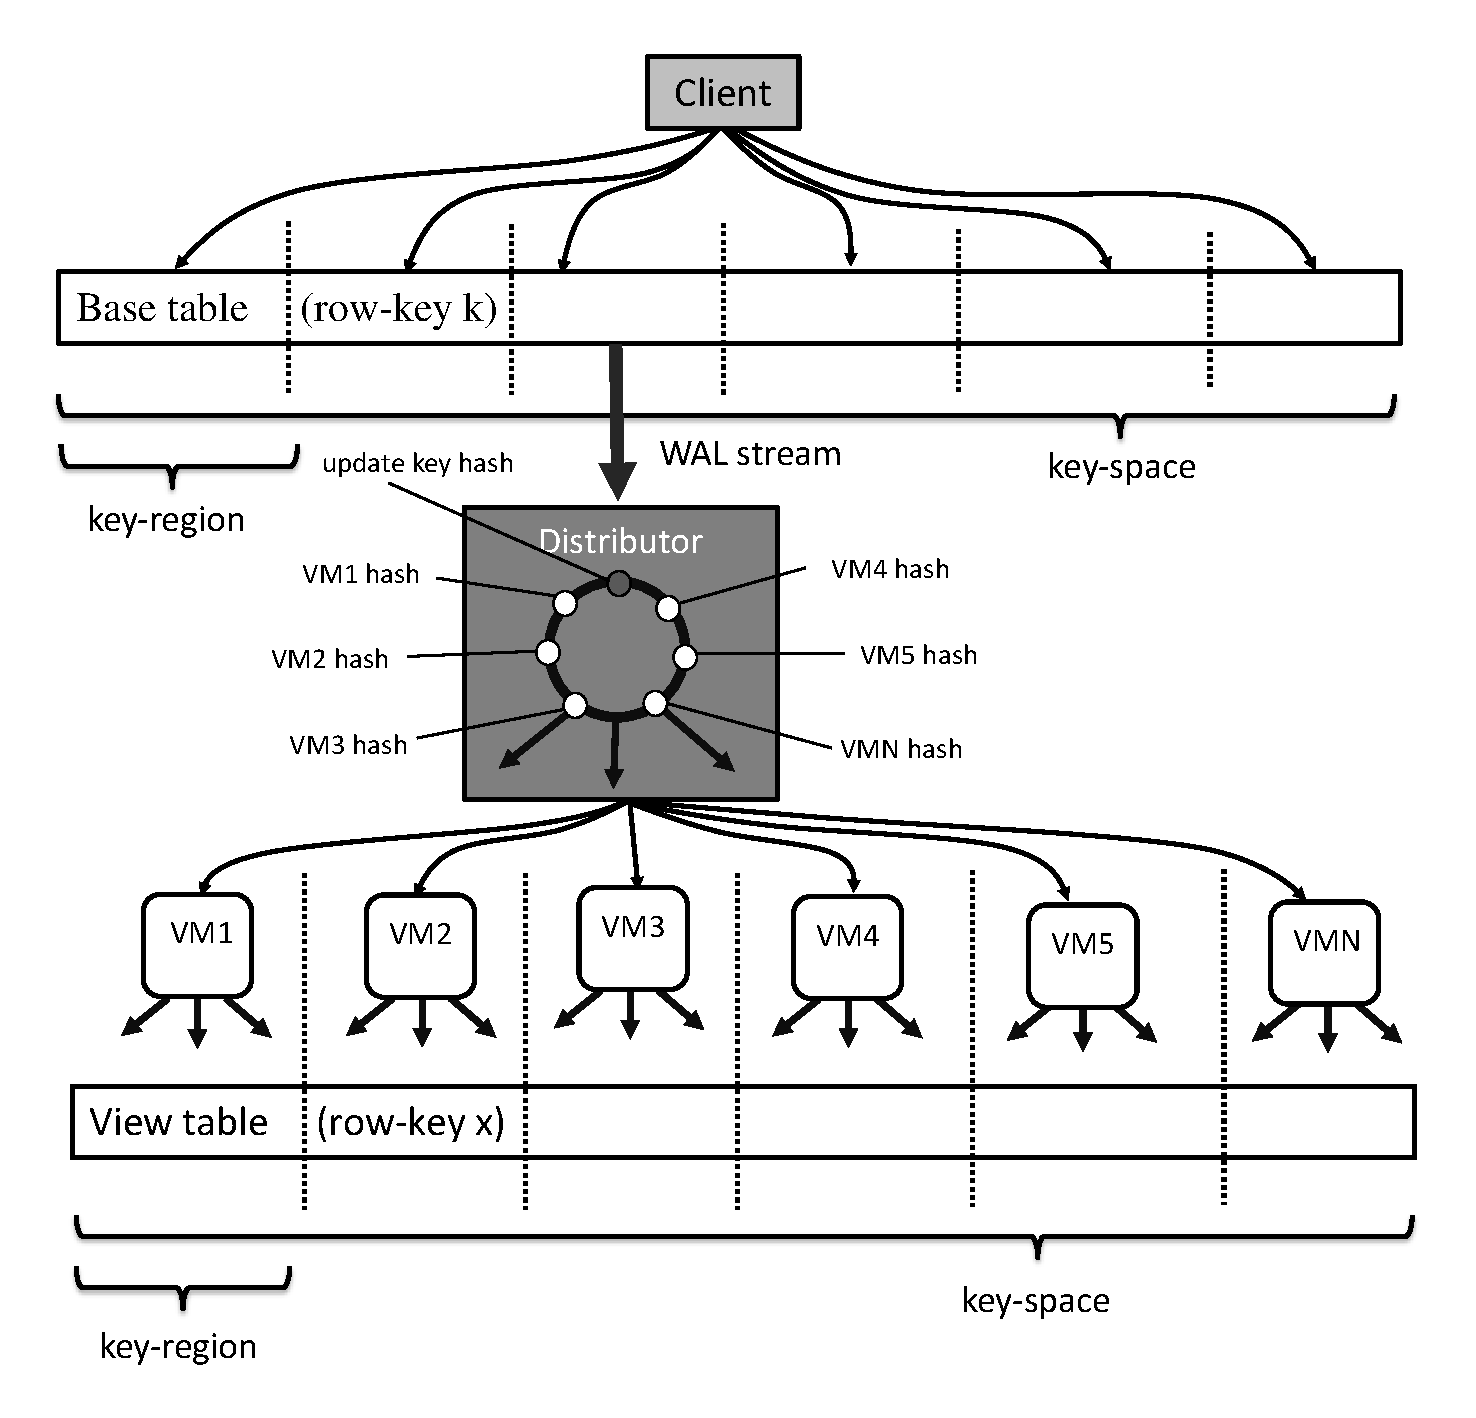
\includegraphics[width=\linewidth]{figures/Consistency}
    \caption{Update distribution through Consistent Hashing}
    \label{fig:review_consistency}
    \vspace{-2mm}
\end{figure}


%\subsubsection{Management Actions and Consistency} 
%
%We now refine the behaviour of \VMS\ to allow for dynamic state
%changes in sub-systems.  For reasons of recovery, load balancing and
%scaling, \VMS\ performs the following actions: \textit{add}, makes the
%\VM\ resource available to the \VMS; \textit{remove}, takes away a
%\VM\ resource; \textit{assign}, makes a \VM\ available to a sub-system
%such that it can process the sub-system's client operations;
%\textit{withdraw}, takes away a \VM\ from a sub-system (opposite of
%assign); and \textit{re-assign}, re-locates a \VM\ from one sub-system
%to another. Adding a \VM\ to \VMS\ (or removing it) does not affect
%view maintenance. The re-assign action is a combination of withdraw
%and assign. Now, we explain how assign and withdraw actions are
%performed safely (i.e., without interfering with consistency).
%
%%\begin{table}
%%\rowcolors{2}{gray!10}{gray!30}
%%\setlength{\belowrulesep}{0pt}
%%\setlength{\aboverulesep}{0pt}
%%\setlength\extrarowheight{2pt}
%%\begin{center}
%%\begin{tabular}{l l l}
%%\toprule
%%Component & action & method \\
%%\midrule
%%View Manager & add & \textit{addViewManager()}  \\
%% & remove & \textit{removeViewManager()}    \\
%% & assign & \textit{assignViewManager()}  \\
%% & withdraw & \textit{withdrawViewManager()}    \\
%% & re-assign & \textit{reassignViewManager()}    \\
%%\bottomrule 
%%\end{tabular}
%%\caption{\VMS\ actions}
%%\label{tab:vms_events}
%%\end{center}
%%\end{table}
%
%%Recall, that the sub-system selects the 
%%responsible \VM\ by applying the hash function. The operation is then 
%%inserted into the corresponding queue. 
%
%
%\noindent
%\textbf{Assign VM:} Figure~\ref{fig:review_consistency} shows how a
%sub-system does view maintenance. Assume a new \VM\ (in the figure
%represented by $V_3$) is assigned to the sub-system. The logic,
%performed on the sub-system during the command, can be described as a
%sequence of primitive actions: (1) Method $createQueue(vm)$ creates a
%queue for a new \VM. (2) The \VM\ is added to the hash-ring by method
%$insertHash(vm)$.  (3) The method $activateQueue(vm)$ starts the
%sending thread that keeps transferring the queue's operations to the
%\VM.
%
%When a \VM\ is assigned, it is inserted into the hash-ring of the 
%sub-system. Unless the hash-ring is empty, the new \VM\ is assigned a key 
%range that is, at the same time, removed from another \VM. This leads
%to violation of consistency (even convergence in terms of the consistency
%model), as the following example shows.
%
%
%\begin{algorithm}
%\caption{Safe assignment procedure at sub-system}
%\label{alg:assignvm}
%\begin{algorithmic}
%\Procedure{$assignVm$}{$vm_a, VM_{sub}$}
%\State{$createQueue(vm_a)$}
%\State{$insertHash(vm_a)$}
%\ForAll{$vm \in VM_{sub}$}
%\State{$queue(vm, m_a)$}\Comment{queue markers}	
%\EndFor
%\ForAll{$vm \in VM_{sub}$}
%\State{$receiveAck(vm)$}\Comment{wait for acks}		
%\EndFor
%\State{$activateQueue(vm_a)$}	
%\EndProcedure
%\end{algorithmic}
%\end{algorithm}
%
%
%\textit{Example}: In Figure~\ref{fig:review_consistency}, $VM_1$ and
%$VM_2$ are already assigned to the sub-system. They are responsible
%for a certain range on the hash-ring; queues are feeding them with
%incoming client operations. Assume a client performing a put operation
%$p_1(k_1, \{..\})$; the sub-system receives $p_1$, selects $VM_2$ as
%responsible and inserts $p_1$ into the queue of $VM_2$.  Now assume, a
%new \VM\ $VM_3$ is assigned to the sub-system and its hash is inserted
%within the range of $VM_2$ such that it acquires the responsibility
%for key $k_1$. In a next step, a client sends an operation $p_2(k_1,
%\{..\})$ to the same key. Because responsibility has changed, the
%operation is sent to $VM_3$. Considering that $VM_3$ has just been
%added, it's queue is empty and, hence, processes updates very fast. It
%is likely to happen that $VM_3$ processes $p_2$ before $VM_2$ can
%process $p_1$. Because both operations refer to the same base record,
%the timeline of the record is broken and convergence is violated.
%
%To process the assign command safely, we use so called \textit{markers}. 
%Markers are -- just like client operations -- enqueued to a \VM\ and 
%become a part of the operation stream. When the \VM, while processing 
%operations, notices a marker, it replies with an acknowledgement back to 
%the sub-system. Thus, the marker reveals to the sub-system, whether the \VM\ 
%has completed all operations that were sent before the marker. We change the 
%assignment procedure by adding a marker-based acknowledgement mechanism 
%(cf. Algorithm~\ref{alg:assignvm}). 
%
%%The
%%algorithm is executed synchronously and if another assignment
%%procedure is called on the sub-system, it must wait, until the first
%%operation has terminated.
%The procedure $assignVm$ takes two parameters: $vm_a$, the \VM\ that 
%should be assigned to the sub-system, and $VM_{sub}$, a set of \VMs\ 
%that are already assigned to the sub-system. The algorithm creates a 
%queue for $vm_a$ and inserts it into the hash-ring. Then, it queues a 
%marker $m_a$ to all assigned \VMs\ ($VM_{sub}$). After the sub-system 
%has received acknowledgements from all \VMs, it is guaranteed that no 
%operation in the key range of the newly added \VM\ $vm_a$ is still 
%pending. Referring back to the above example: The timeline of $k_1$ can 
%not be changed any more. 
%
%%Operation $t_2$ has to
%%wait in the queue of $VM_3$ until $VM_2$ acknowledges the processing
%%of $t_1$ because the queue of $VM_3$ is activated only after the
%%marker has been acknowledged and this, in turn, implies that operation
%%$t_1$ has been processed.
%\noindent
%\textbf{Withdraw VM:} The logic, performed on the sub-system side
%during a withdraw can be described analogously to the assign command
%by a sequence of primitives (opposite actions in reverse order): (1)
%$deactivateQueue(vm)$ stops the sending thread that keeps transferring
%the operations in the queue to the \VM. (2) The \VM\ is removed from
%the hash-ring by $removeHash(vm)$. (3) $deleteQueue(vm)$ removes the
%queue for the withdrawn \VM. The queue can only be deleted, if it is
%empty and no operation is queued.
%
%\begin{algorithm}
%\caption{Safe withdraw procedure at sub-system}
%\label{alg:withdrawvm}
%\begin{algorithmic}
%\Procedure{$withdrawVm$}{$vm_w, VM_{sub}$}
%\ForAll{$vm \in VM_{sub} \wedge vm \neq vm_w$}	
%\State{$deactivateQueue(vm)$}
%\EndFor
%\State{$removeHash(vm_w)$}
%\State{$queue(vm_w, m_w)$}\Comment{queue marker}
%%\ForAll{$vm \in VM_{sub}$}
%\State{$receiveAck(vm_w)$}\Comment{wait for ack}		
%%\EndFor
%\State{$removeQueue(vm_w)$}
%\ForAll{$vm \in VM$}
%\State{$activateQueue(vm)$}
%\EndFor
%\EndProcedure
%\end{algorithmic}
%\end{algorithm}
%
%    
%Also, during a withdraw procedure, consistency may be violated. At the
%moment where a \VM\ is withdrawn, i.e., removed from the hash-ring,
%its queue might still contain operations. If another \VM\ that
%acquires the key range is fast enough, it might processes operations
%before the withdrawn \VM\ has finished. Again, the timeline of base
%records is changed. In order to prevent inconsistencies, we designed
%Algorithm~\ref{alg:withdrawvm} analogously to
%Algorithm~\ref{alg:assignvm}. It takes two parameters: $vm_w$, the
%\VM\ that should be withdrawn from the sub-system, and $VM_{sub}$, the
%set of \VMs\ that is assigned to the sub-system.
%
%First, the queues of the \VMs\ that possibly increase their key range
%on the hash-ring (i.e., all other \VMs) are deactivated. Then, a
%marker $m_w$ is queued at the \VM\ that is withdrawn. If the \VM\ has
%acknowledged the marker, the sub-system knows, that all operations
%have been processed. It removes the queue of the \VM\ and re-activates
%the queues of all \VMs.
%

\subsection{Consistency}
\label{sec:consistency}

Since consistency is a major concern during incremental view maintenance 
-- additionally, we introduce a high degree of concurrency -- we now 
show, how the fundamentals of Section~\ref{subsec:consistency_model} 
influence the \VMS\ design. As a first step, we discuss the three rules
of Theorem~1, separately.


%we define a consistency model before building the VMS. 
%In data warehouse environments, for batch-based view update
%processing, consistency models have been extensively explored (e.g.,
%~\cite{zhuge:view, wang:efficient, zhang:parallel, zhuge:strobe}. For
%view maintenance in KV-stores a model has been proposed
%in~\cite{jacobsen:viewmaintenance}. First, we adapt this model and the
%corresponding consistency levels to match the characteristics of 
%KV-stores (defined in the previous section). Second, we define a theorem, 
%capturing the requirements against our VMS, in order to achieve strong
%consistency.



\subsubsection{Exactly once property}
\label{subsubsec:exactly_once}  

Like stated in our theorem, Rule~1, updating a view exactly once for 
every client operation is critical, as views can be non-idempotent. 
There are two possible incidents that 
violate the exactly once requirement: an operation is lost (maybe due to 
node crash, or transmission errors); an operation is applied 
more than once (in consequence of a log replay after a node crash). 
In either case, the view would be incorrect (i.e., does not converge).

One architectural decision of VMS was to read the update operations from
the WAL of the \KVS\ node. Updates in the WAL are persisted safely and
replicated via HDFS. Even though a node or a \VM goes down and update 
operations are lost, they can be always recovered from the WAL of the 
\KVS\ node. Actually, the WAL serves the same purpose for the \KVS\ itself.
As soon as a node crashes, the \KVS replays all transactions that have 
not been flushed to the table file before and would have been lost otherwise.


As updates cannot be lost, the \VMS\ guarantees an at-most-once semantic.
Still, we need to assure that updates in \VMS\ are not duplicated. In case a crash 
occurs, the WAL reader may re-process some of 
the updates and send them to the \VMs\ a second time. Then, the \VM\ needs 
to identify the duplicate and drop it. We achieve the identification of
duplicates with the help of a global ID (i.e. signature); this ID can only 
be obtained from the \KVS, as the update operations originate from here. 
Our implementation builds on top of \HB, a global ID can be created by 
combining an operations sequence number and the node ID. This ID is delivered
with every update operation. The \VM\ just keeps track of the highest maintained
operation ID (this information can be stored into Zookeeper, as the system is 
fault-tolerant). If ever an operation with a lower ID is sent to the \VM, it 
identifies the duplicate and drops it.




\subsubsection{Atomic view record update}
\label{subsubsec:atomic_update} 

Like stated in our theorem, Rule~2, every view update has to be executed 
atomically. Regarding a view update, we rely on the semantics that are 
provided by \KVS. We assume (as it is the case for \HB\ and \CAS) that a 
single put or delete operation, e.g. $put(k_1, \langle c_1, x_1\rangle, 
\langle c_2, 10\rangle)$, is executed ACID compliant. Thus, a row update 
has to be atomic; the \KVS\ is not allowed to execute let's say 
$put(k_1, \langle c_1, x_1\rangle)$ and then $put(k_1, \langle c_2, 
10\rangle)$ later. 


Despite the single update operation (i.e. get/put), also the complete 
update process -- comprising of a get-operation to the old view record 
and a put/delete- operation to the new view record -- has to be ACID 
compliant. Most view types define a mapping from multiple base table 
records to a single view table record (e.g. aggregation). As shown in 
Example~2 different base table records may be propagated to different 
VMs, multiple VMs can concurrently update the same view record. 
Remembering the execution alternatives from 
Subsection~\ref{subsec:update_processing}, this problem has to be 
solved, differently. 




\noindent
\textbf{Alternative~1:} Distributing the update operation according to the
base table row-key means, there could be multiple \VM, updating one view
table row-key. For example put operations $put(k_1, \langle c_1, x_1\rangle, 
\langle c_2, 10\rangle)$ and $put(k_5, \langle c_1, x_1\rangle, \langle c_2, 
5\rangle)$ could be forwarded to different \VMs, still both \VMs have to
access row key $x_1$. To solve the problem, we use test-And-set methods to 
avoid interruption during updates. The \VM\ retrieves the old view record,
e.g. $(x_1, \langle c_{sum},20\rangle)$ and extracts one of the values (here,
it is the aggregation value $20$). When updating and writing back the new 
value, e.g. $25$, the \VM\ sends a test-and-set request to the server with
a test-value (here $20$). 


\noindent
\textbf{Alternative~2:} Distributing the update operation according to the 
hash of the view table row-key completely eliminates the need of further 
synchronization mechanisms. Every \VM\ is responsible for an equal amount
of view table records and, thus, for a part of the view table. As there is 
no ambiguity, \VMs\ can just use regular get and put/delete operations.


%\noindent
%\textit{Example~3:} Given base table $A(\underline{K}, F)$ and a \texttt{SUM} 
%view $S(\underline{X}, F)$, defined as $S=\gamma_{c_1,Sum(c_2)}(A)$. 
%Assume a client inserts two records into base table $A$. The KV-store writes the following 
%operations into the transaction log: $t_1=put(k_1,\{\langle 
%c_1,x_1\rangle,\langle c_2,a\rangle\})$ and $t_2=put(k_2, \{\langle 
%c_1,x_1 \rangle,\linebreak \langle c_2,b\rangle\})$. Let the VMS receive both 
%operations and process them in parallel. To perform view maintenance, 
%the VMS retrieves the corresponding old view records from the view 
%table. Since $S$ is a \texttt{SUM} view -- and $t_1$ and $t_2$ refer to 
%the same aggregation key $x_1$ -- the VMS retrieves the same view record 
%twice, e.g. $(x_1, \{\langle c_s, v_s\rangle\})$. In case of $t_1$ VMS 
%adds the delta $a$ to the view record; in case of $t_2$ VMS adds the 
%delta $b$. Then, the VMS writes the updated view records back to the 
%view table. Depending on which record is written first, the VMS 
%overwrites one update with the other. Say, VMS writes $(x_1, \{\langle 
%c_s, v_s+a \rangle\})$ to $S$; then it overwrites the result with 
%$(x_1,\{\langle c_s, v_c+b\rangle\})$. In consequence the delta $a$ is 
%missing in the view. The correct result should be $(x_1,\{\langle c_s, 
%v_s+a+b \rangle\})$. Therefore, atomic view updates are essential. 
%


%In our implementation, we use a test-and-set mechanism to solve this
%problem.~\footnote{In HBase a \texttt{checkAndPut} method is provided
%  to realize this mechanism. Most KV-stores offer a similar
%  abstraction.} When updating a table record, a caller sees (tests)
%whether a record has been concurrently modified between a read and an
%update.
%
%Revisiting Example~2, let $VM_2$ retrieve value $(x1, \{(col_1,
%a)\})$. Then, it computes $(x1,\{(col_1,a+c)\})$ trying to put the new
%value, while testing for the old value $a$. The test-and-set fails
%because the old record value changed concurrently to $a+b$. Thus,
%$VM_2$ fetches the updated value again and re-computes
%$(x1,\{(col_1,a+b+c)\})$. This time the test-and-set succeeds and the
%record is written.

\subsubsection{Record timeline}
\label{subsubsec:record_timeline} 

Record timeline means that sequences of operations on the same row key are not re-ordered 
when processed by VMS.  Again, a little example demonstrates the
importance of record timeline semantics.


\noindent
\textbf{Alternative~1:} Distributing the update operation according to the
base table row-key means, time-line of a record cannot be broken. All 
operations that touch a specific row-key will always be directed to the 
same \VM; they will be retrieved in-order,  sent to the \VM\ in-order and
updated in the view in-order.
%
%there could be multiple \VM, updating one view
%table row-key. For example put operations $put(k_1, \langle c_1, x_1\rangle, 
%\langle c_2, 10\rangle)$ and $put(k_5, \langle c_1, x_1\rangle, \langle c_2, 
%5\rangle)$ could be forwarded to different \VMs, still both \VMs have to
%access row key $x_1$. To solve the problem, we use test-And-set methods to 
%avoid interruption during updates. The \VM\ retrieves the old view record,
%e.g. $(x_1, \langle c_{sum},20\rangle)$ and extracts one of the values (here,
%it is the aggregation value $20$). When updating and writing back the new 
%value, e.g. $25$, the \VM\ sends a test-and-set request to the server with
%a test-value (here $20$). 


\noindent
\textbf{Alternative~2:} Distributing the update operation according to the 
hash of the view table row-key also creates a record timeline. But in 
contrast to Alternative~1, it is the timeline of the view table, which
bears the following consequences: As long as the view table record doesn't
change, updates to the same base table row-key are also forwarded to the 
same \VM.  As soon as an update modifies the view table row-key -- which means
the update touches two records in one view table -- the timeline
of the base table row-key could be broken. 

For that reason, we need a mechanism which prevents this scenario. We 
employ a buffer for update operations. But only for those updates, that 
change the view table key in question -- insert and delete operations, 
as well as update operations that don't change the key are processed 
just like before; matching this criterion, the update is inserted into the 
buffer, send to a \VM, where it causes the old entry to be deleted; 
it is, then, deleted from the buffer and passed to another \VM, where it 
causes the new entry to be inserted. If during that process, however, more
updates flow in 




\subsubsection{Conclusion}
\label{subsubsec:conclusion} 

In the previous sections, we described two alternatives and their implications.
Both alternatives have their up- and downsides. Alternative~1 supports the 
preservation of base record time-line, whereas Alternative~2 supports the 
concurrent access to the view table. Both alternatives are convenient consistency
concepts, in both cases the implementation needs to be complemented with
additional mechanisms (i.e. test-and-Set methods, update buffer) to achieve
strong consistency. 

Still, we favor Alternative~2 over Alternative~1. One reason is the fact that
Alternative~1 uses Test-And-Set methods. Even though it is a pessimistic locking
mechanism -- in contrast to optimistic locking, a view record is always accessible --
it is not suited well in our case \footnote{Actually, modern system try to avoid locking completely} 
for the following reasons: (1) If there is high contention, a lot of view updates have
to be repeatedly applied, (2) we have to use test-and-set for every view update,
despite of it being an insert, update or delete, which introduces overhead. 
In contrast, we choose Alternative~2 for the following reasons: (1) it is a 
locking-free alternative (most state-of-the-art transaction systems use locking-free
mechanisms). (2) The update buffer is only needed for a small fraction of update
operations (i.e. not for inserts, not for deletes, etc..). Thus performance overhead
is minimal.





\subsubsection{Nested constructions}
\label{subsubsec:nested_constructions} 

So far, we have only discussed the simple case, with one base and one view
table. As we strive for support of more complex constructs (i.e. SQL-like 
queries) in \VMS, we need to extend our design.

\begin{figure}
  \centering
    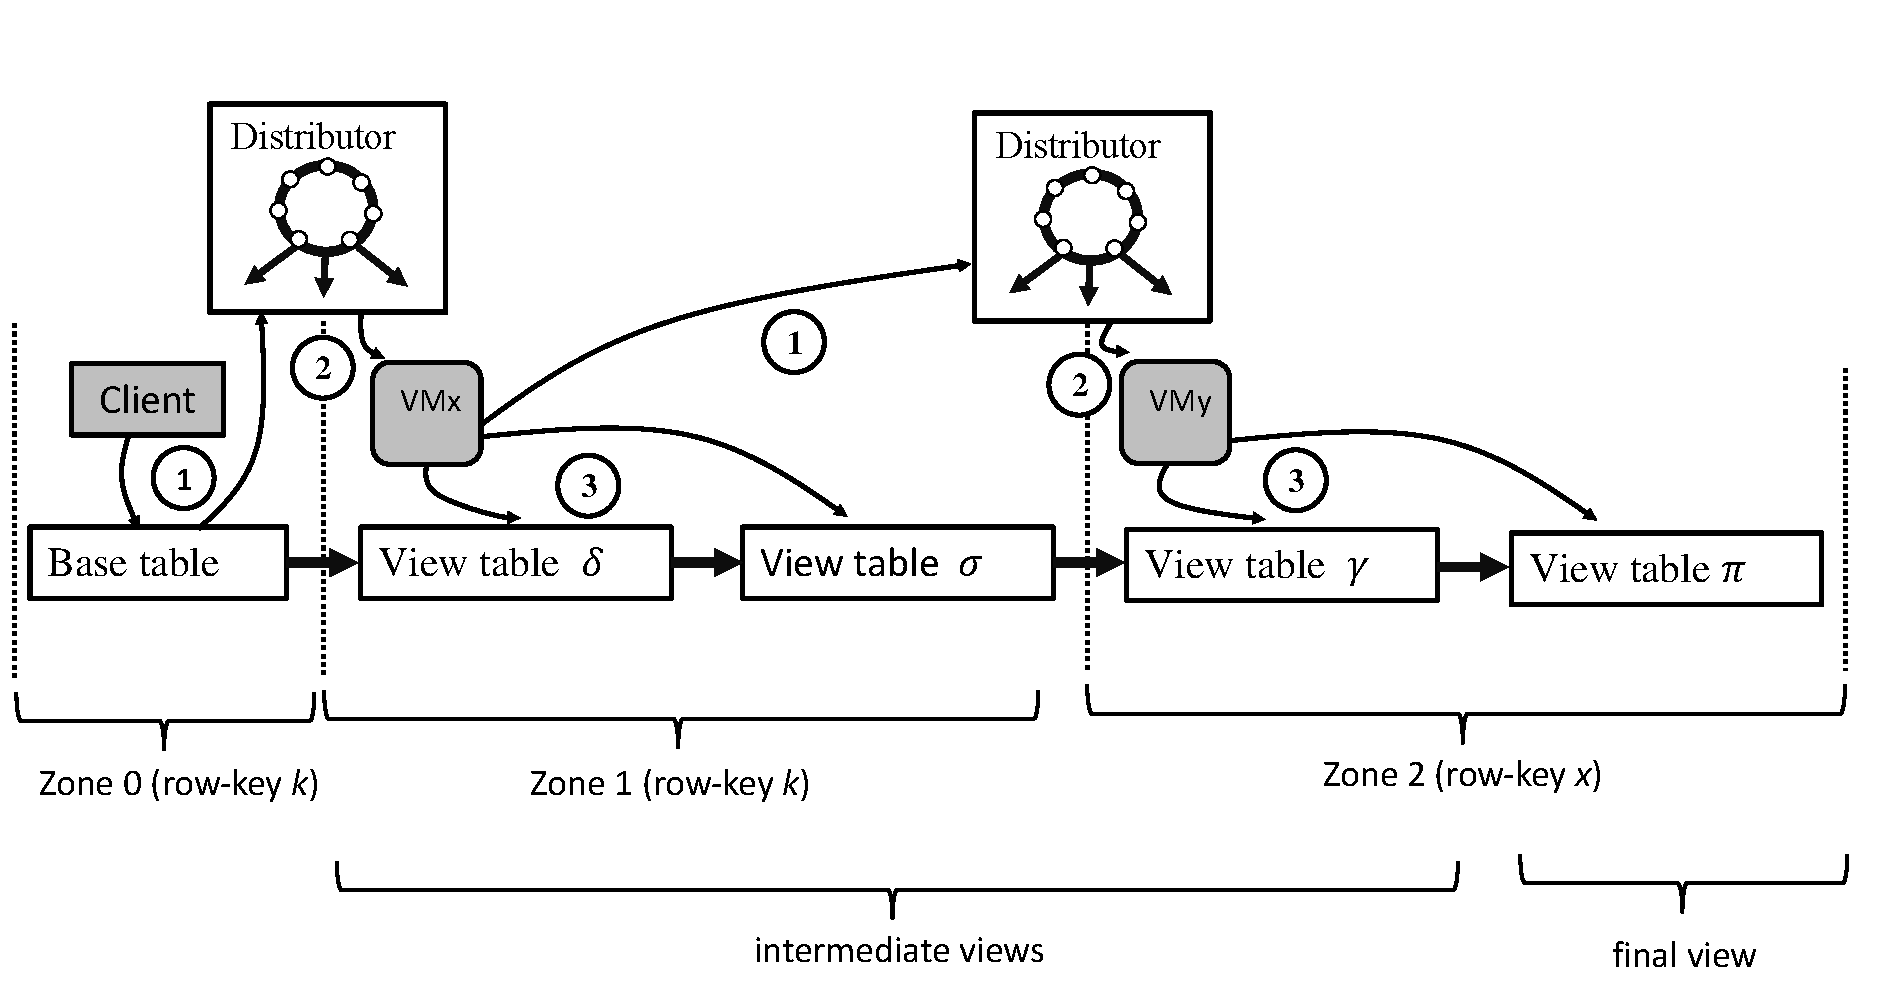
\includegraphics[width=\linewidth]{figures/Concept}
    \caption{Executing a query with views}
    \label{fig:view_concept}
    \vspace{-2mm}
\end{figure}

Usually, a query consists of multiple clauses (e.g. select, from, where, 
group by). In order to translate the query, we need to build a 
maintenance plan. This can be done with the help of a directed acyclic 
graph (DAG); each node in the DAG represents one materialized view. 
Starting from the base table, all views are inter-connected and each 
pair of view tables resembles a base/view table-relation. The moment a 
base table gets updated, the operation travels subsequently to all views 
and updates them incrementally. The result of the query can be obtained 
from the last view. 



In Figure~\ref{fig:view_concept}, the maintenance process of the 
following query is depicted: $\text{Select }sum(c2)\text{ from 
}bt1\text{ group by }c1\text{ where }c2\:<\:10$ It can be observed that 
the update path is divided into two \textit{zones}. A zone describes a 
part of the update path where all views possess the same row key. To improve
performance, a \VM\ can update the view tables of a zone in one run. 
Once a zone 
-- and therefore also the row key -- changes, updates need to be 
re-distributed in order to sustain consistency (cf. 
Figure~\ref{fig:review_consistency}). In the figure two zones can be 
identified. The maintenance of a zone is always processed in a cycle of 
three steps: 


\begin{enumerate}
	\item Update is provided to distributor
	\item Update is assigned and sent to VM
	\item Update is applied to view tables of zone
\end{enumerate} 


In the first step, the update operation is provided to the distributor
component of the source system. During maintenance of the first zone
the update is provided by the WAL reader of the source system itself, 
during maintenance of subsequent zones, it is provided by the last 
responsible \VM. In the second step, the distributor assigns and 
distributes updates as described above (cf. Figure~\ref{fig:view_concept}).
In the third step, the \VM\ goes along the path of each view table in
the zone, retrieves the old view record, updates it incrementally and 
stores the new version back into the view. Then the cycle is repeated
for every zone. As all the updates of a zone can are distributed 
according to the cardinality of the row key, a high parallelisation of 
updates can be achieved.


%\subsection{Proof of Consistency}


Theorem~\ref{theo:strong_consistency} states that a VMS system fulfilling all 
three requirements achieves at least strong consistency. In the following, we 
will present a proof for this theorem, which is organized in three stages: we 
start with proving convergence and then present extensions to also prove weak 
consistency  and finally strong consistency.





\subsubsection{Notation}
First, we define the following notation for keys, 
operations on keys, and the ordering of operations. Let $k_x$ denote a key in 
a base table, where $x \in X = \{1, \dots, m\}$, and $X$ is the 
table's key range. Further, let an operation on key $k_x$ be defined as 
$t[k_x]$, and a totally ordered sequence of such operations be denoted by 
$\langle t_1, t_2, t_{3}, \dots, t_N\rangle$, where $N$ defines the total 
number of operations on the table in a given timespan. 
Hence, a generalized sequence of operations on a base table is 
represented by $\langle t_1[k_{x_1}], t_2[k_{x_2}], \dots, 
t_n[k_{x_m}]\rangle$, where $k_{x_1}, \dots, k_{x_m} \in X$ can be arbitrarily 
chosen from the base table's key range for every timestamp. Based on this 
generalized sequence every other sequence of operations can be derived, e.g. 
$\langle t_1[k_{1}],t_2[k_{2}],t_3[k_{1}]\rangle$. In some cases, we also want 
to keep the ordering of operations variable. For that reason, we introduce an 
index $s_i$ with $i \in \{1, \dots, n\}$. Then we can write the arbitrary 
sequence as $\langle t_{s_1}[k_{x_1}], t_{s_2}[k_{x_2}], \dots, 
t_{s_n}[k_{x_n}]\rangle$ with $s_1\neq \dots \neq s_n$. Using this notion, we 
are capable of representing every possible sequence of update operations in 
the system. 

The index $t^{(i)}[k_x]$ is used to express a sequence of operations on 
a single row key (i.e. the time-line). For example, a sequence of 
operations on row key $k_x$ is denoted as $\langle 
t^{(1)}[k_x],t^{(2)}[k_x]...,t^{( \omega)}[k_x]\rangle$. The last 
operation on a particular row key is always denoted with $\omega$. (see 
Section~\ref{sec:consistency}).

For the proof, we assume such an arbitrary sequence of base table operations
 and then we show that --- given the requirements in the theorem --- a VMS 
 system will produce correct view results. Formally, we show that $V_f=View(B_f)$. 

\subsubsection{Convergence}
\label{sub:proof_convergence}
As mentioned earlier, every view type defines its own mapping from base table 
to view table records. Thus, we prove the different cases separately. 

\noindent
\textit{One-to-one mapping:} \texttt{SELECTION}, \texttt{PROJECTION} 
views define a one-to-one mapping between base and view table. The row 
key of the base table is also the row key of the view table. Operations 
for both view types are idempotent, meaning an operation could be 
applied several times without changing the result. The view record is 
always a representation of the last base table operation applied. A 
correct view record with row key $k$ is defined as the last operation on 
the row key in the base table key, e.g. $k\leftarrow 
View(t^{(\omega)}[k])$. The function $View$ calculates the view record 
(by using the appropriate view definition) and applies the result to the 
correct view key. A view table converges, if all view records are 
computed correctly in the last view state. 

We start defining an arbitrary sequence of operations on the base table, 
shown in Step~\ref{proof:oo_step1}. Clients can update different row 
keys in the base table, using put or delete operations. Likewise, they 
can update the same row key multiple times. The update operations of the 
clients form a particular global order, expressed through $t_1..t_n$. 
They take the base table from its initial state $B_0$ to its final state 
$B_f$. In the next step, all update operations get forwarded, causing 
the ordering of operations to be lost. If we would continue working with 
an unordered set, convergence of the view will be violated at some 
point. For this reason, we apply requirement (iii) (,i.e. the time-line 
requirement) to our equation, as depicted in Step~\ref{proof:oo_step3}. 
As updates operations do not influence each other (see requirement 
(ii)), we are able to create a set of sub-sequences. These 
sub-sequences only consist of updates that have been applied to the same 
row key. Likewise the sub-sequences contain all operations from the 
previous step (see requirement (i)). 
%
\begin{subequations}
  \begin{align}
 S_b&=\langle t_1[k_{x_1}],....,t_n[k_{x_n}] \rangle;\;\;\Big(B_0 \overset{S_b}{\rightarrow}B_f\Big) \label{proof:oo_step1}\\ 
 S_1&=\langle t^{(1)}[k_{1}],..,t^{(\omega_1)}[k_{1}]\rangle,..,S_m=\langle t^{(1)}[k_{m}],..,t^{(\omega_m)}[k_{m}]\rangle\label{proof:oo_step3}\\
  S_1&=\langle t^{(\omega_1)}[k_{1}]\rangle,..,S_m=\langle t^{(\omega_m)}[k_{m}]\rangle\label{proof:oo_step4}\\
 S_v&=\langle t_{s_1}^{(\omega_1)}[k_{1}],..t_{s_n}^{(\omega_m)}[k_{m}]\rangle;\; \Big(V_0\overset{S_v}{\rightarrow}V_f\Big)\label{proof:oo_step5}\\
 	V_f&=k_x\leftarrow View(t^{(\omega_x)}[k_x])=View(B_f)\label{proof:oo_step6}
  \end{align}
\end{subequations}
%
In Step~\ref{proof:oo_step4}, we pick the last element of all 
sub-sequences and eliminate the rest. As stated above, only the last 
operation on a particular row key has an influence on the final view 
state. Again, we observe that the time-line of a row key is vital. If it 
is broken, e.g. for row key $k_1$, then an operation 
$t^{(\omega-1)}[k_{1}]$ can be incorporated into the final result and 
render it incorrect. After the elimination, we unite the operations 
again in Step~\ref{proof:oo_step5}. The reunion allows the remaining 
operations to be executed in every possible order (i.e. every operation 
could be executed in parallel). Finally, the view definition is applied 
to every operation in $R$. This leads to the correct final view records 
and hence, to convergence. The \texttt{DELTA} view also defines a 
one-to-one mapping between base and view records. In contrast to the 
aforementioned views, the results of the \texttt{DELTA} view do not only 
relate to the last, but to the two last operations. Therefore, we need 
to change the last three steps of the proof as follows: 
%
\begin{subequations}
  \begin{align}
  S_1&=\langle t^{(\omega_1-1)}[k_{1}],t^{(\omega_1)}[k_{1}]\rangle,..,S_m=\langle t^{(\omega_m-1)}[k_{m}],t^{(\omega_m)}[k_{m}]\rangle\\
   S_v&=\langle t_{s_1}^{(\omega_1-1)}[k_{1}],t_{s_2}^{(\omega_1)}[k_{1}],..t_{s_{n-1}}^{(\omega_m-1)}[k_{m}],t_{s_n}^{(\omega_m)}[k_{m}]\rangle\label{proof:ood_step2}\\
   &(\forall t_{s_i}^{(\omega_y-1)}\in S_v)(\exists t_{s_j}^{(\omega_y)}\in S_v)\;s_i < s_j;\;\Big(V_0\overset{S_v}{\rightarrow}V_f\Big)\notag\\
 	V_f&=k_x\leftarrow View(t^{(\omega_x-1)}[k_x],t^{(\omega_x)}[k_x])=View(B_f)
  \end{align}
\end{subequations}
%
As can be observed in Step~\ref{proof:ood_step2}, the two last 
operations of a time-line are included into the final result. However, 
the sequence can be arbitrarily ordered, but needs to preserve the 
time-line of both last operations (i.e. $\omega-1$ must always precede 
$\omega$). Computing $V_f$ leads to the valid final state and the 
\texttt{DELTA} view converges. 

\noindent
\textit{Many-to-one mapping:} (\texttt{PRE}-)\texttt{AGGREGATION} and 
\texttt{INDEX} views define a many-to-one mapping between base and view 
table. The row key of the view table is the aggregation key. Multiple 
row keys in the base table can relate to a particular aggregation key. 
However, a base table row has always only one aggregation key. A correct 
view record with aggregation key $x$ is defined as the combination of 
multiple base records $k_{x_1}..k_{x_j}$, related to the particular key. 
In terms of incremental view maintenance, the correct view record can be 
defined as a number of last operations, that have been applied to this 
combination of base records: $x \leftarrow 
View(t^{(\omega_1)}[k_{x_1}],..,t^{(\omega_j)}[k_{x_j}])$. In case of a 
\texttt{SUM} view e.g., this resolves to $x \leftarrow 
f(t^{(\omega_1)}[k_1])+..+f(t^{(\omega_j)}[k_j])$. We start again, 
defining an arbitrary sequence of base table operations in 
Step~\ref{proof:mo_step1}. In contrast to the previously handled views, 
we are now processing $\delta$-operations. We construct a number of $m$ 
sub- sequences, each containing the $\delta$-operations of one 
particular base record key. In Step~\ref{proof:mo_step2}, we merge the 
$\delta$-operations together. All $\delta$- operations add up to form 
the last transaction as the end result (i.e. $\delta(t^{(1)}[k_{1}])+
..+\delta(t^{( \omega_1)}[k_{1}])=t^{(\omega_1)}[k_{1}]$). 
%\begin{subequations}
%  \begin{align}
%  \{t_1(k_1),..,t_n(k_1)..t_1(k_n),..,t_n(k_n)\}\\
% \{\langle t_1(k_1),..,t_n(k_1)\rangle,..\langle t_1(k_n),..,t_n(k_n)\rangle\}\\
% \{\langle t_n(k_1)\rangle,..\langle t_n(k_n)\rangle\}\\
% 	x=f(t_n(k_1))+..+f(t_n(k_n))
%  \end{align}
%\end{subequations}
%
\begin{subequations}
  \begin{align}
  S_b&=\langle t_1[k_{x_1}],....,t_n[k_{x_n}] \rangle;\;\Big(B_0 \overset{S_b}{\rightarrow}B_f\Big) \label{proof:mo_step1}\\ 
 S_1&=\langle \delta(t^{(1)}[k_{1}]),.,\delta(t^{(\omega_1)}[k_{1}])\rangle,..,\label{proof:mo_step2}\\
 &\hspace{10 mm}S_m=\langle \delta(t^{(1)}[k_{m}]),.,\delta(t^{(\omega_m)}[k_{m}])\rangle\notag\\
  S_1&=\langle t^{(\omega_1)}[k_{1}]\rangle,..,S_m=\langle t^{(\omega_m)}[k_{m}]\rangle\\
 S_v&=\langle t_{s_1}^{(\omega_1)}[k_{1}],..t_{s_n}^{(\omega_m)}[k_{m}]\rangle;\;\Big(V_0\overset{S_v}{\rightarrow}V_f\Big)\label{proof:mo_step4}\\
 	V_f&=x\leftarrow View(t^{(\omega_{x_1})}[k_{x_1}],.., t^{(\omega_{x_j})}[k_{x_j}])=View(B_f)\label{proof:mo_step5}
 	%&\hspace{10 mm}x_1,..,x_j \in \{1,..,m\};\;x_1\neq,..,\neq x_j \notag
  \end{align}
\end{subequations}
%
Now, we can unite the single sequences as done before. We retrieve a 
final sequence as shown in Step~\ref{proof:mo_step4}. The operations of 
this sequence are then applied to the view --- simultaneously they are 
grouped and stored according to their aggregation key. The final view 
records are calculated correctly, as depicted in 
Step~\ref{proof:mo_step5}, which causes the aggregation view to 
converge. 

\textit{Many-to-many mapping:} (\texttt{REVERSE}-)\texttt{JOIN} views 
define a many-to-many mapping between base and view table. The row key 
of the view table is a composite key of both join tables' row key. 
Multiple records of both base tables form a set of multiple view records 
in the view table. Since the joining of tables takes place in the 
\texttt{REVERSE JOIN} view, we prove convergence only for this view 
type. A \texttt{REVERSE JOIN} view has a structure that is similar to an 
aggregation view. The row key of the \texttt{REVERSE JOIN} view is the 
join key of both tables. All base table records are grouped according to 
this join key. But in contrast to an aggregation view the 
\texttt{REVERSE JOIN} view combines two base tables to create one view 
table. A correct view record with join key $x$ is defined as a 
combination of operations on keys $k_1..k_n$ from join table $A$ and 
operations on keys $l_1..l_p$ from join table $B$. In order to represent 
both keys we introduce an additional variable $z_1,..,z_n \in 
\{k_1,..,k_m, l_1,..,l_p\}$. Then, the correct view record is defined 
as: $x \leftarrow View(t^{(\omega_1)}[z_1], ..,t^{(\omega_j)}[z_j])$. 
We start with a sequence of arbitrary client updates to both base 
tables, as depicted in Step~\ref{proof:mm_step1}. Then, the order of 
updates is lost and the time-line requirement is realized in 
Step~\ref{proof:mm_step2}. 
%
\begin{subequations}
  \begin{align}
  S_b&=\langle t_1[z_1],..,t_n[z_n]\rangle;\;\Big(B_0 \overset{S_b}{\rightarrow}B_f\Big)\label{proof:mm_step1}\\ 
 S_1&=\langle \delta(t^{(1)}[k_{1}]),..,\delta(t^{(\omega_1)}[k_{1}])\rangle,..,S_m,..,S_{m+1},..\label{proof:mm_step2}\\ 
&\hspace{10 mm}S_{m+p}=\langle \delta(t^{(1)}[l_{p}]),..,\delta(t^{(\omega_p)}[l_{p}])\rangle\notag\\
  S_1&=\langle t^{(\omega_{k_1})}[k_{1}]\rangle,.., S_m=\langle t^{(\omega_{k_m})}[k_{m}]\rangle,..,\\
 &\hspace{10 mm}S_{m+1}=\langle t^{(\omega_{l_1})}[l_{1}]\rangle,..,S_{m+p}=\langle t^{(\omega_{l_p})}[l_{p}]\rangle\notag\\
 S_v&=\langle t^{(\omega_{k_1})}[k_{1}],..t^{(\omega_{k_m})}[k_{m}],\\
 &\hspace{10 mm}t^{(\omega_{l_1})}[l_{1}],..,t^{(\omega_{l_p})}[l_{p}] \rangle;\;\Big(V_0\overset{S_v}{\rightarrow}V_f\Big)\label{proof:mm_step3}\\
 	V_f&=x\leftarrow View(t^{(\omega_{z_1})}[z_1],.., t^{(\omega_{z_j})}[z_j])=View(B_f)\label{proof:mm_step4}
 	%&\hspace{10 mm}z_1,..,z_j \in \{k_1,..,k_m,l_1,..,l_p\}; z_1\neq,..,\neq z_j ;\; \notag
  \end{align}
\end{subequations}
%
We eliminate all but the last operations $\omega$ and reunite the 
operations in Step~\ref{proof:mm_step3}. This leads to the final 
Step~\ref{proof:mm_step4}, where the operations are applied to the view 
record. Since the view records are calculated correctly (i.e. only the 
last operations of the row keys are included) we conclude that the view 
converges. 

\subsubsection{Weak consistency} 
\label{sub:proof_weak}

Weak consistency has been defined as follows: Weak consistency is given 
if the view converges and all intermediary view states are valid, 
meaning they can be derived from one of the base states with 
$V_j=View(B_i)$. As we already proved convergence, we need show that all 
the intermediary view states are correct likewise. We start again with 
an arbitrary sequence of operations in Step~\ref{proofw:oo_step1}. In 
order to generate an intermediate base state, we cut the sequence at any 
point before an operation $t_a$, with $1 < a < n$. After the ordering is 
lost, we apply the time-line consistency. But in contrast to before, we 
are not capable of processing the complete time-line (i.e. 
$(1)..(\omega)$). Instead, we process the time-line until an 
intermediary element $\alpha_x \leq \omega_x$. 
%
\begin{subequations}
  \begin{align}
  S_b&=\langle t_1[k_{x_1}],....,t_n[k_{x_n}] \rangle;\;\Big(B_0 \overset{S_b}{\rightarrow}B_{a}\Big)\label{proofw:oo_step1}\\
 S_1&=\langle t^{(1)}[k_{1}],..,t^{(\alpha_1)}[k_{1}]\rangle,..,S_m=\langle t^{(1)}[k_{m}],..,t^{(\alpha_m)}[k_{m}]\rangle\\
 S_v&=\langle t_{s_1}^{(1)}[k_{1}],..t_{s_i}^{(\alpha_1)}[k_{1}],..,t_{s_j}^{(1)}[k_{m}],..,t_{s_a}^{(\alpha_m)}[k_{m}]\rangle;\;\Big(V_0\overset{S_v}{\rightarrow}V_a\Big)\\
 (\forall& t_{s_1}^{(\lambda_1)}[k_{x_1}] \in S_v)(\forall t_{s_2}^{(\lambda_2)}[k_{x_2}] \in S_v):(x_1=x_2)\;\land\;(\lambda_1<\lambda_2) \Rightarrow s_1 < s_2\notag\\
V_{a}&=k_x\leftarrow View(t^{(\alpha_x)}[k_x])=View(B_{\alpha})
  \end{align}
\end{subequations}


\subsubsection{Strong consistency}
\label{sub:proof_strong}

Strong consistency has been defined as follows: Weak consistency is 
achieved and the following conditions hold true. All pairs of view 
states $V_i$ and $V_j$ that are in a relation $V_i \leq V_j$ are derived 
from base states $Bi$ and $B_j$ that are also in a relation $B_i \leq 
B_j$. Since weak consistency is already proven, we only need to prove 
the statement $V_i \leq V_j \Rightarrow B_i \leq B_j$. If this statement 
is negated, then only two of the following cases can occur: Either $V_i 
\leq V_j \Rightarrow B_i \parallel B_j$ or $V_i \leq V_j \Rightarrow B_i 
\geq B_j$. Both cases can only be constructed by breaking the record 
time-line. To be precise: At least one record has to exists, whose 
time-line is broken. Formally, we demand $ (\exists t_l \in B_i)(\forall 
t_k \in B_j):(r(t_l)=r(t_k))\land(l > k) $. Because requirement (iv) 
prevents the breaking of time-lines, we conclude that both cases are not 
possible. Thus, we have proven strong consistency by contradiction. 


%
%\subsubsection{Local processing}
%
%Record timeline means that updates of the same row key are not re-ordered 
%when processed by the system. 


%We consider the following scenarios. Execution of two operations on
%the same row key, $k_1$ and two operations on different row keys,
%$k_1$ and $k_2$. We distinguish between one client $c_1$ sending both
%operations in sequence versus two clients $c_1$ and $c_2$ concurrently
%sending one each. This gives rise to four cases, covering all possible
%input orderings of two operations (i.e., possible base table update
%sequences). Let the base table be defined as $A(\underline{K},\{F\})$.
%
%\noindent
%Client $\boldsymbol{c_1}$ updates $\boldsymbol{k_1}$,
%$\boldsymbol{k_1}$ (1): The client performs two operations
%$t_1=put(A(k_1,\allowbreak\{\langle c_1,v_1\rangle\}))$ followed by
%$t_2=put(A(k_1,\{\langle c_2,v_2\rangle\}))$ to the same base table
%record. Client operations via the KV-API are synchronous and happen in
%order. For that reason, the node writes $t_1$ to its TL followed by
%$t_2$. Given that the NX reads the TL sequentially, it processes both
%operations in order. For each $t_i$ ($i = 1, 2$), NX selects a VM$_1$
%by computing the hash $h(k_i)$, where it queues the operation.  As
%assumed, the row keys of $t_1$ and $t_2$ are the same, so for both
%operations the same VM is selected, where the view updates are
%processed in order by calling on the synchronous KV-API for view table
%updates.
%
% 
%
%\noindent
%Clients $\boldsymbol{c_1}$, $\boldsymbol{c_2}$ update
%$\boldsymbol{k_1}$ (2): Let client $c_1$ perform $t_1$ and client
%$c_2$ perform $t_2$ (both operations on the same row key). Both
%clients connect to the KV-API and are routed to the same node. Since
%the KV-store executes put operations atomically, and locks a record
%during the operation, one client operation always precedes the
%other. Therefore, the order of $t_1$ and $t_2$ is determined by
%whichever operation happens to be processed first, leading to its
%insertion into the TL. When retrieving $t_1$ and $t_2$, the NX
%computes the hash of the corresponding keys, as above.  Thus, the same
%VM is selected in both cases. Therefore, the order of two updates, on
%the same record, by different clients, is determined by the KV-store;
%subsequently, the order is not changed by VMS.
%
%Based on this analysis, we conclude that VMS maintains record timeline
%consistency for view updates. However, we analysed timeline 
%consistency with regard to a static set-up of view managers. We 
%assumed that the number of VMs per node remains fix during the 
%maintenance process. If we introduce load balancing mechanisms or 
%add new view managers to the system on-the-fly, then we need to review 
%the guarantee of timeline consistency. This is done in the appendix, 
%Section~\ref{sec:dynamic_scalability}.
%
%\begin{algorithm}
%\caption{Operation processing at VM}
%\label{alg:processing}
%\begin{algorithmic}[5]
%\Procedure{$processOperation$}{$t \in T$}%\Comment{$t$ received from NX}
%\State $bt \leftarrow getBaseTable(t)$%\Comment{lookup meta table}	
%\State $V \leftarrow resolveViewDefinitions(bt)$%\Comment{lookup meta table}		
%\ForAll{$v \in V$}
%\While{$\neg succeed$}	
%\State $vt \leftarrow getViewTable(v)$
%\State $vk \leftarrow getViewKey(t, v)$	%\Comment{extract view key}	
%\State $vr' \leftarrow KVStore.get(vt, vk)$
%\State $sig \leftarrow getSignature(t)$%\Comment{retrieve signature}
%\If{$vr' \neq null\wedge hasProcessed(vr', sig)$}
%\State $break$%\Comment{leave if $t$ already processed}	
%\EndIf
%\State $vr \leftarrow computeUpdate(vr', t)$\label{line:compute_update}
%\State $suceed \leftarrow KVStore.checkAndPut(vt, vk, vr', vr)$\label{line:check_and_put}
%\EndWhile %\Comment{retry until view updated}
%\State $writeCommitLog(vt)$
%\EndFor
%\EndProcedure
%\end{algorithmic}
%\end{algorithm}
%%
%
%Algorithm~\ref{alg:processing} shows the general steps a VM executes as
%it propagates updates.  It includes the test-and-set and the signature
%mechanism described above.  The former is realized via the
%\texttt{checkAndPut} method available in HBase, for example.  Thus,
%Algorithm~\ref{alg:processing} enforces the exactly once and the
%atomic update propagation requirements. However, preservance of view record
%timeline semantic is enforced by the design of VMS.


%\subsubsection{Fault-tolerance} 
%
%Failure detection and recovery play a critical role in \VMS.  In this
%section, we analyse the behaviour of \VMS\ under \VM\ and node crashes
%to ensure that after appropriate recovery measures, views still
%converge.
%
%\noindent
%\textbf{\VM\ crash} -- A \VM\ maintains a queue with operations
%dispatched to it. During a \VM\ crash, these operations are lost, which
%may result in non-converging views. Our recovery measures described
%here, ensure view convergence under \VM\ crash. A \VM\ crash triggers an
%event via ZooKeeper, notifying the \VMS\ coordinator.
%
%First, the coordinator sends a withdraw command to the concerned
%sub-system. The sub-system withdraws the crashed \VM\ from the
%hash-ring and stops dispatching operations to it. This way no updates,
%that were in-fight, while the \VM\ crashed, are lost. Next, the
%coordinator starts a new \VM\ instance. Upon start-up, it tells the
%new \VM\ to replay the \VM-log of the crashed \VM. The new
%\VM\ contacts ZooKeeper and retrieves the last processed sequence
%number of the crashed
%\VM\ (cf. Section~\ref{subsec:update_processing}).  The new
%\VM\ accesses the \VM\ log of the crashed \VM\ and -- starting from
%the sequence number -- replays all the entries.
%
%\noindent
%\textbf{Node crash} -- A node crash is handled by the recovery
%mechanism of the \KVS. The \KVS\ moves all key ranges of the crashed
%node to other nodes. In case, client operations exist that were just
%residing in memstore (and had not been written to the table file), the
%\KVS\ replays the\TL. During replay, all operations are inserted into
%memstore and directly flushed to disk.
%
%The \TL\ of a crashed node is still available (due to replication in
%the underlying file system, HDFS, for example.) Thus, the sub-system
%that is streaming the operations from the crashed node's
%\TL\ continues reading to the end of file. Now, that the stream (of
%the crashed node's \TL) runs dry, \VMS\ re-assigns all \VMs\ to a
%different sub-system.
%
%Based on the above reasoning, we conclude that \VMS\ is able to
%prevent loss and duplication of operations during crashes.
